% Options for packages loaded elsewhere
\PassOptionsToPackage{unicode}{hyperref}
\PassOptionsToPackage{hyphens}{url}
%
\documentclass[
]{article}
\usepackage{amsmath,amssymb}
\usepackage{iftex}
\ifPDFTeX
  \usepackage[T1]{fontenc}
  \usepackage[utf8]{inputenc}
  \usepackage{textcomp} % provide euro and other symbols
\else % if luatex or xetex
  \usepackage{unicode-math} % this also loads fontspec
  \defaultfontfeatures{Scale=MatchLowercase}
  \defaultfontfeatures[\rmfamily]{Ligatures=TeX,Scale=1}
\fi
\usepackage{lmodern}
\ifPDFTeX\else
  % xetex/luatex font selection
\fi
% Use upquote if available, for straight quotes in verbatim environments
\IfFileExists{upquote.sty}{\usepackage{upquote}}{}
\IfFileExists{microtype.sty}{% use microtype if available
  \usepackage[]{microtype}
  \UseMicrotypeSet[protrusion]{basicmath} % disable protrusion for tt fonts
}{}
\makeatletter
\@ifundefined{KOMAClassName}{% if non-KOMA class
  \IfFileExists{parskip.sty}{%
    \usepackage{parskip}
  }{% else
    \setlength{\parindent}{0pt}
    \setlength{\parskip}{6pt plus 2pt minus 1pt}}
}{% if KOMA class
  \KOMAoptions{parskip=half}}
\makeatother
\usepackage{xcolor}
\usepackage[margin=1in]{geometry}
\usepackage{color}
\usepackage{fancyvrb}
\newcommand{\VerbBar}{|}
\newcommand{\VERB}{\Verb[commandchars=\\\{\}]}
\DefineVerbatimEnvironment{Highlighting}{Verbatim}{commandchars=\\\{\}}
% Add ',fontsize=\small' for more characters per line
\usepackage{framed}
\definecolor{shadecolor}{RGB}{248,248,248}
\newenvironment{Shaded}{\begin{snugshade}}{\end{snugshade}}
\newcommand{\AlertTok}[1]{\textcolor[rgb]{0.94,0.16,0.16}{#1}}
\newcommand{\AnnotationTok}[1]{\textcolor[rgb]{0.56,0.35,0.01}{\textbf{\textit{#1}}}}
\newcommand{\AttributeTok}[1]{\textcolor[rgb]{0.13,0.29,0.53}{#1}}
\newcommand{\BaseNTok}[1]{\textcolor[rgb]{0.00,0.00,0.81}{#1}}
\newcommand{\BuiltInTok}[1]{#1}
\newcommand{\CharTok}[1]{\textcolor[rgb]{0.31,0.60,0.02}{#1}}
\newcommand{\CommentTok}[1]{\textcolor[rgb]{0.56,0.35,0.01}{\textit{#1}}}
\newcommand{\CommentVarTok}[1]{\textcolor[rgb]{0.56,0.35,0.01}{\textbf{\textit{#1}}}}
\newcommand{\ConstantTok}[1]{\textcolor[rgb]{0.56,0.35,0.01}{#1}}
\newcommand{\ControlFlowTok}[1]{\textcolor[rgb]{0.13,0.29,0.53}{\textbf{#1}}}
\newcommand{\DataTypeTok}[1]{\textcolor[rgb]{0.13,0.29,0.53}{#1}}
\newcommand{\DecValTok}[1]{\textcolor[rgb]{0.00,0.00,0.81}{#1}}
\newcommand{\DocumentationTok}[1]{\textcolor[rgb]{0.56,0.35,0.01}{\textbf{\textit{#1}}}}
\newcommand{\ErrorTok}[1]{\textcolor[rgb]{0.64,0.00,0.00}{\textbf{#1}}}
\newcommand{\ExtensionTok}[1]{#1}
\newcommand{\FloatTok}[1]{\textcolor[rgb]{0.00,0.00,0.81}{#1}}
\newcommand{\FunctionTok}[1]{\textcolor[rgb]{0.13,0.29,0.53}{\textbf{#1}}}
\newcommand{\ImportTok}[1]{#1}
\newcommand{\InformationTok}[1]{\textcolor[rgb]{0.56,0.35,0.01}{\textbf{\textit{#1}}}}
\newcommand{\KeywordTok}[1]{\textcolor[rgb]{0.13,0.29,0.53}{\textbf{#1}}}
\newcommand{\NormalTok}[1]{#1}
\newcommand{\OperatorTok}[1]{\textcolor[rgb]{0.81,0.36,0.00}{\textbf{#1}}}
\newcommand{\OtherTok}[1]{\textcolor[rgb]{0.56,0.35,0.01}{#1}}
\newcommand{\PreprocessorTok}[1]{\textcolor[rgb]{0.56,0.35,0.01}{\textit{#1}}}
\newcommand{\RegionMarkerTok}[1]{#1}
\newcommand{\SpecialCharTok}[1]{\textcolor[rgb]{0.81,0.36,0.00}{\textbf{#1}}}
\newcommand{\SpecialStringTok}[1]{\textcolor[rgb]{0.31,0.60,0.02}{#1}}
\newcommand{\StringTok}[1]{\textcolor[rgb]{0.31,0.60,0.02}{#1}}
\newcommand{\VariableTok}[1]{\textcolor[rgb]{0.00,0.00,0.00}{#1}}
\newcommand{\VerbatimStringTok}[1]{\textcolor[rgb]{0.31,0.60,0.02}{#1}}
\newcommand{\WarningTok}[1]{\textcolor[rgb]{0.56,0.35,0.01}{\textbf{\textit{#1}}}}
\usepackage{longtable,booktabs,array}
\usepackage{calc} % for calculating minipage widths
% Correct order of tables after \paragraph or \subparagraph
\usepackage{etoolbox}
\makeatletter
\patchcmd\longtable{\par}{\if@noskipsec\mbox{}\fi\par}{}{}
\makeatother
% Allow footnotes in longtable head/foot
\IfFileExists{footnotehyper.sty}{\usepackage{footnotehyper}}{\usepackage{footnote}}
\makesavenoteenv{longtable}
\usepackage{graphicx}
\makeatletter
\def\maxwidth{\ifdim\Gin@nat@width>\linewidth\linewidth\else\Gin@nat@width\fi}
\def\maxheight{\ifdim\Gin@nat@height>\textheight\textheight\else\Gin@nat@height\fi}
\makeatother
% Scale images if necessary, so that they will not overflow the page
% margins by default, and it is still possible to overwrite the defaults
% using explicit options in \includegraphics[width, height, ...]{}
\setkeys{Gin}{width=\maxwidth,height=\maxheight,keepaspectratio}
% Set default figure placement to htbp
\makeatletter
\def\fps@figure{htbp}
\makeatother
\setlength{\emergencystretch}{3em} % prevent overfull lines
\providecommand{\tightlist}{%
  \setlength{\itemsep}{0pt}\setlength{\parskip}{0pt}}
\setcounter{secnumdepth}{-\maxdimen} % remove section numbering
\newlength{\cslhangindent}
\setlength{\cslhangindent}{1.5em}
\newlength{\csllabelwidth}
\setlength{\csllabelwidth}{3em}
\newlength{\cslentryspacingunit} % times entry-spacing
\setlength{\cslentryspacingunit}{\parskip}
\newenvironment{CSLReferences}[2] % #1 hanging-ident, #2 entry spacing
 {% don't indent paragraphs
  \setlength{\parindent}{0pt}
  % turn on hanging indent if param 1 is 1
  \ifodd #1
  \let\oldpar\par
  \def\par{\hangindent=\cslhangindent\oldpar}
  \fi
  % set entry spacing
  \setlength{\parskip}{#2\cslentryspacingunit}
 }%
 {}
\usepackage{calc}
\newcommand{\CSLBlock}[1]{#1\hfill\break}
\newcommand{\CSLLeftMargin}[1]{\parbox[t]{\csllabelwidth}{#1}}
\newcommand{\CSLRightInline}[1]{\parbox[t]{\linewidth - \csllabelwidth}{#1}\break}
\newcommand{\CSLIndent}[1]{\hspace{\cslhangindent}#1}
\ifLuaTeX
  \usepackage{selnolig}  % disable illegal ligatures
\fi
\IfFileExists{bookmark.sty}{\usepackage{bookmark}}{\usepackage{hyperref}}
\IfFileExists{xurl.sty}{\usepackage{xurl}}{} % add URL line breaks if available
\urlstyle{same}
\hypersetup{
  pdftitle={Probability Distributions},
  pdfauthor={Giovanni Saraceno},
  hidelinks,
  pdfcreator={LaTeX via pandoc}}

\title{Probability Distributions}
\author{Giovanni Saraceno}
\date{}

\begin{document}
\maketitle

{
\setcounter{tocdepth}{2}
\tableofcontents
}
\hypertarget{probability-distributions}{%
\section{Probability Distributions}\label{probability-distributions}}

The concepts of probability and randomness are central to statistics. In
particular, to understand statistical methods, it is important to view
data as samples derived from distributions.

This section outlines the basic ideas of probability and functions in
\texttt{R} for random sampling and handling theoretical distributions.

\hypertarget{random-sampling}{%
\subsection{Random Sampling}\label{random-sampling}}

Early examples in probability theory primarily dealt with gambling and
games where the core concept was random sampling, such as shuffling a
deck of cards or drawing numbered balls. In \texttt{R}, we can simulate
such situations using the \texttt{sample} function. For example, to draw
5 numbers (randomly!) from the set \texttt{1:90}, we can use:

\begin{Shaded}
\begin{Highlighting}[]
\FunctionTok{sample}\NormalTok{(}\DecValTok{1}\SpecialCharTok{:}\DecValTok{90}\NormalTok{, }\DecValTok{5}\NormalTok{)}
\end{Highlighting}
\end{Shaded}

\begin{verbatim}
## [1]  4 28 72 39 46
\end{verbatim}

The first argument, \texttt{x}, is a vector indicating the set to sample
from, while \texttt{size} specifies the sample size. By default, the
sample function samples \textbf{without replacement} (i.e., the sample
cannot contain duplicate values), so the sample size cannot exceed the
length of the set. To sample \textbf{with replacement}, use the option
\texttt{replace\ =\ TRUE}. For example, to simulate 10 coin tosses:

\begin{Shaded}
\begin{Highlighting}[]
\FunctionTok{sample}\NormalTok{(}\FunctionTok{c}\NormalTok{(}\StringTok{"H"}\NormalTok{, }\StringTok{"T"}\NormalTok{), }\DecValTok{10}\NormalTok{, }\AttributeTok{replace =} \ConstantTok{TRUE}\NormalTok{)}
\end{Highlighting}
\end{Shaded}

\begin{verbatim}
##  [1] "H" "H" "H" "T" "H" "H" "T" "H" "T" "H"
\end{verbatim}

In a fair coin toss, the events ``Heads'' and ``Tails'' are equally
likely (i.e., each has a probability of \(\frac{1}{2}\)). In R, we can
also consider cases where the events are not equally probable using the
\texttt{prob} option:

\begin{Shaded}
\begin{Highlighting}[]
\FunctionTok{sample}\NormalTok{(}\FunctionTok{c}\NormalTok{(}\StringTok{"H"}\NormalTok{, }\StringTok{"T"}\NormalTok{), }\DecValTok{10}\NormalTok{, }\AttributeTok{replace =} \ConstantTok{TRUE}\NormalTok{, }\AttributeTok{prob =} \FunctionTok{c}\NormalTok{(}\FloatTok{0.9}\NormalTok{, }\FloatTok{0.1}\NormalTok{))}
\end{Highlighting}
\end{Shaded}

\begin{verbatim}
##  [1] "H" "H" "H" "H" "H" "H" "H" "H" "H" "H"
\end{verbatim}

\textbf{Note}: The sum of the values in the prob vector must equal 1.

\hypertarget{combinatorics}{%
\subsection{Combinatorics}\label{combinatorics}}

Consider the example of sampling 5 numbers without replacement. The
probability of a specific number being drawn first is \(\frac{1}{90}\),
for the second \(\frac{1}{89}\), and so on. Thus, the probability of a
specific sample is:

\begin{Shaded}
\begin{Highlighting}[]
\DecValTok{1} \SpecialCharTok{/} \FunctionTok{prod}\NormalTok{(}\DecValTok{90}\SpecialCharTok{:}\DecValTok{86}\NormalTok{)}
\end{Highlighting}
\end{Shaded}

\begin{verbatim}
## [1] 1.896126e-10
\end{verbatim}

This is the probability of drawing specific numbers. If this scenario
corresponds to a lottery, we are interested in the probability of
guessing a specific set of 5 numbers. In this case, we must account for
all possible orders of the 5 numbers, which is \(5!\) or
\(5 \times 4 \times 3 \times 2 \times 1\). The probability of winning
the lottery is:

\begin{Shaded}
\begin{Highlighting}[]
\FunctionTok{factorial}\NormalTok{(}\DecValTok{5}\NormalTok{) }\SpecialCharTok{/} \FunctionTok{prod}\NormalTok{(}\DecValTok{90}\SpecialCharTok{:}\DecValTok{86}\NormalTok{)}
\end{Highlighting}
\end{Shaded}

\begin{verbatim}
## [1] 2.275351e-08
\end{verbatim}

Alternatively, we can calculate the total number of ways to choose 5
elements from 90 using the binomial coefficient:
\[\binom{90}{5} = \frac{90!}{5! 85!} = 43949268\] In R, we use the
choose function:

\begin{Shaded}
\begin{Highlighting}[]
\DecValTok{1} \SpecialCharTok{/} \FunctionTok{choose}\NormalTok{(}\DecValTok{90}\NormalTok{, }\DecValTok{5}\NormalTok{)}
\end{Highlighting}
\end{Shaded}

\begin{verbatim}
## [1] 2.275351e-08
\end{verbatim}

\hypertarget{distributions-in-r}{%
\subsection{Distributions in R}\label{distributions-in-r}}

Consider independent replications of a given experiment. From a
probabilistic perspective, we are often less interested in individual
outcomes and more focused on the total number of outcomes. This result
is random and thus described by a random variable.\\
\textbf{Remark}: A \emph{random variable} is a real-valued function from
an outcome space into the real line more generally into \(R^n\) . The
probability law defined on the outcome space induces (defines
explicitly) a probability model for the random variable. It is the basic
quantity used in probability theory to characterize a probability
process. Random variables are categorized as discrete or continuous.

A discrete random variable \(X\) takes values in a finite set and is
characterized by its probability mass function \(f(x) = P(X = x)\) or
its cumulative distribution function \(F(x) = P(X \leq x)\).

A (uni-variate) continuous random variable can take values in the real
line and is characterized by its density function \(f(x)\) and
distribution function (or cumulative distribution function):
\[F(x) = \int_{-\infty}^x f(x) dx\] \texttt{R} includes implementations
of major probability distributions, both discrete and continuous, as
these are central to statistical modeling and hypothesis testing
(discussed later), replacing traditional statistical tables. Examples
include:

\begin{longtable}[]{@{}ll@{}}
\toprule\noalign{}
\textbf{Distribution} & \textbf{R Name} \\
\midrule\noalign{}
\endhead
\bottomrule\noalign{}
\endlastfoot
Binomial & \texttt{binomial} \\
Chi-squared & \texttt{chisq} \\
Exponential & \texttt{exp} \\
Geometric & \texttt{geom} \\
Poisson & \texttt{pois} \\
Normal & \texttt{norm} \\
t-Student & \texttt{t} \\
\end{longtable}

Each distribution allows for four fundamental operations:Probability
density/mass, Cumulative distribution, Quantiles, Random number
generation. By adding a prefix to the distribution name in \texttt{R},
we can compute these quantities:

\begin{longtable}[]{@{}ll@{}}
\toprule\noalign{}
\textbf{prefix} & \textbf{function} \\
\midrule\noalign{}
\endhead
\bottomrule\noalign{}
\endlastfoot
d & Density \\
p & Cumulative distribution \\
q & Quantile \\
r & Random Generation \\
\end{longtable}

\hypertarget{density}{%
\subsubsection{Density}\label{density}}

The density function is rarely used directly but is helpful for
plotting:

\begin{Shaded}
\begin{Highlighting}[]
\NormalTok{x }\OtherTok{\textless{}{-}} \FunctionTok{seq}\NormalTok{(}\SpecialCharTok{{-}}\DecValTok{4}\NormalTok{, }\DecValTok{4}\NormalTok{, }\FloatTok{0.1}\NormalTok{)}
\FunctionTok{plot}\NormalTok{(x, }\FunctionTok{dnorm}\NormalTok{(x), }\AttributeTok{type =} \StringTok{"l"}\NormalTok{)}
\end{Highlighting}
\end{Shaded}

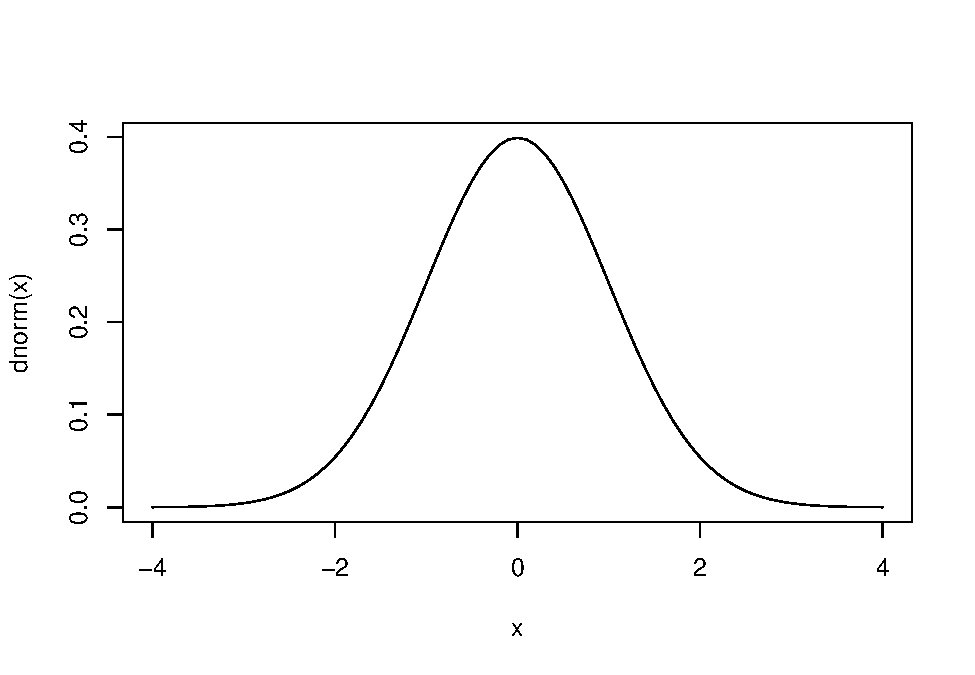
\includegraphics{Probability-Distributions_files/figure-latex/unnamed-chunk-7-1.pdf}
or using \texttt{gggplo2}

\begin{Shaded}
\begin{Highlighting}[]
\FunctionTok{library}\NormalTok{(ggplot2)}
\end{Highlighting}
\end{Shaded}

\begin{verbatim}
## Warning: il pacchetto 'ggplot2' è stato creato con R versione 4.3.3
\end{verbatim}

\begin{Shaded}
\begin{Highlighting}[]
\NormalTok{x }\OtherTok{\textless{}{-}} \FunctionTok{seq}\NormalTok{(}\SpecialCharTok{{-}}\DecValTok{4}\NormalTok{, }\DecValTok{4}\NormalTok{, }\FloatTok{0.1}\NormalTok{)}
\NormalTok{df }\OtherTok{\textless{}{-}} \FunctionTok{data.frame}\NormalTok{(}\AttributeTok{x =}\NormalTok{ x, }\AttributeTok{density =} \FunctionTok{dnorm}\NormalTok{(x))}

\FunctionTok{ggplot}\NormalTok{(df, }\FunctionTok{aes}\NormalTok{(}\AttributeTok{x =}\NormalTok{ x, }\AttributeTok{y =}\NormalTok{ density)) }\SpecialCharTok{+}
  \FunctionTok{geom\_line}\NormalTok{() }\SpecialCharTok{+}
  \FunctionTok{labs}\NormalTok{(}\AttributeTok{title =} \StringTok{"Density of the Standard Normal Distribution"}\NormalTok{,}
       \AttributeTok{x =} \StringTok{"x"}\NormalTok{, }\AttributeTok{y =} \StringTok{"Density"}\NormalTok{) }\SpecialCharTok{+}
  \FunctionTok{theme\_minimal}\NormalTok{()}
\end{Highlighting}
\end{Shaded}

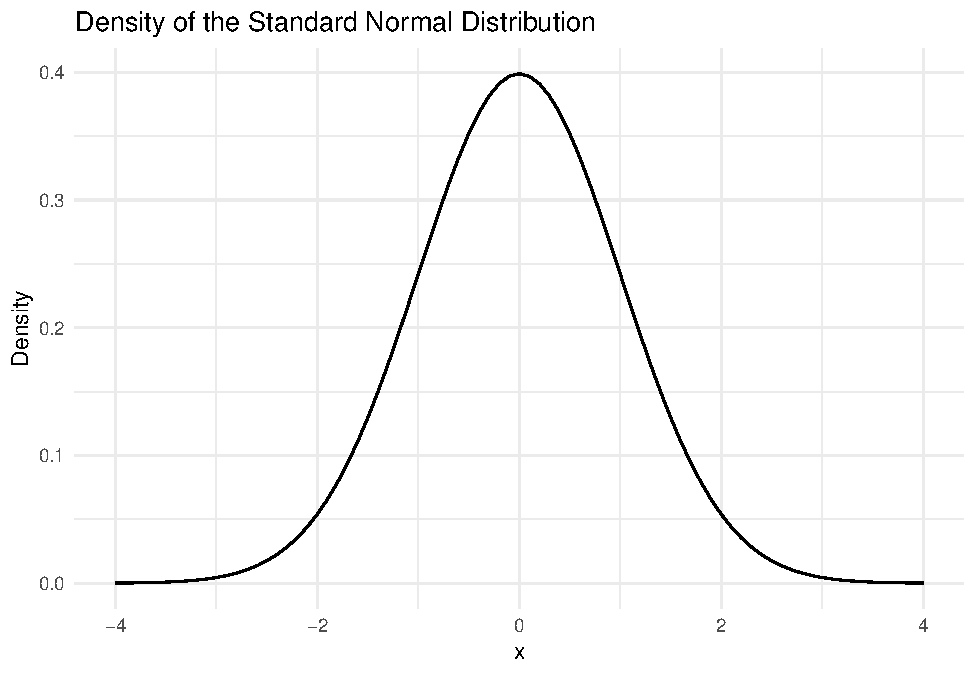
\includegraphics{Probability-Distributions_files/figure-latex/unnamed-chunk-8-1.pdf}

Alternatively, we can use:

\begin{Shaded}
\begin{Highlighting}[]
\FunctionTok{curve}\NormalTok{(}\FunctionTok{dnorm}\NormalTok{(x), }\AttributeTok{from =} \SpecialCharTok{{-}}\DecValTok{4}\NormalTok{, }\AttributeTok{to =} \DecValTok{4}\NormalTok{)}
\end{Highlighting}
\end{Shaded}

For discrete distributions, a ``stick diagram'' is often used. For
example, the binomial distribution with \(n = 40\),\(p=0.3\):

\begin{Shaded}
\begin{Highlighting}[]
\NormalTok{x }\OtherTok{\textless{}{-}} \DecValTok{0}\SpecialCharTok{:}\DecValTok{40}
\NormalTok{df\_binom }\OtherTok{\textless{}{-}} \FunctionTok{data.frame}\NormalTok{(}\AttributeTok{x =}\NormalTok{ x, }\AttributeTok{density =} \FunctionTok{dbinom}\NormalTok{(x, }\AttributeTok{size =} \DecValTok{40}\NormalTok{, }\AttributeTok{prob =} \FloatTok{0.3}\NormalTok{))}
\FunctionTok{plot}\NormalTok{(x, df\_binom}\SpecialCharTok{$}\NormalTok{density, }\AttributeTok{type =} \StringTok{"h"}\NormalTok{)}
\end{Highlighting}
\end{Shaded}

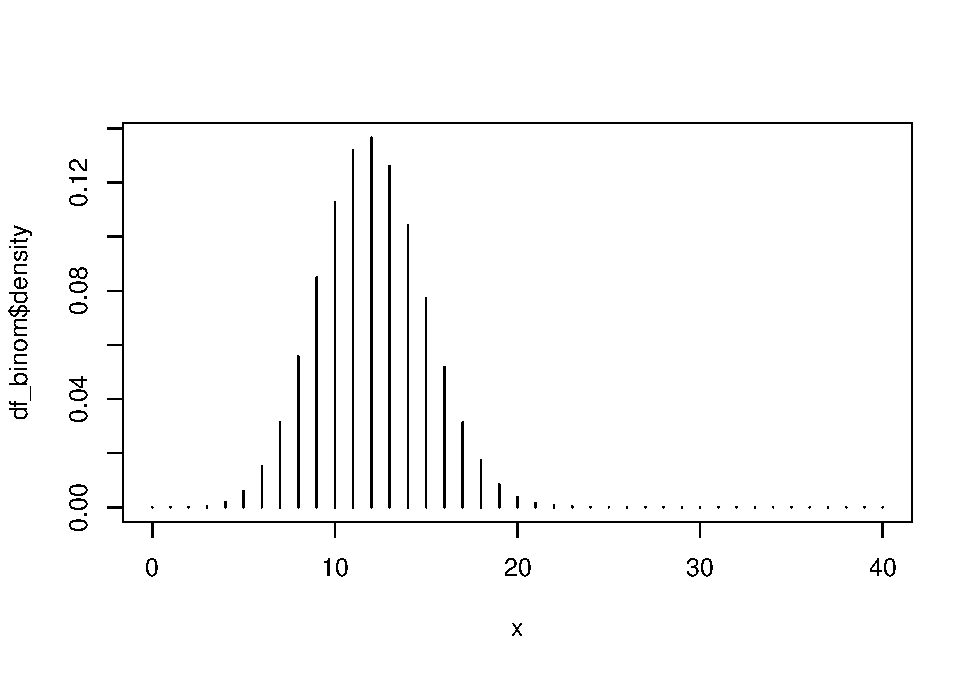
\includegraphics{Probability-Distributions_files/figure-latex/unnamed-chunk-10-1.pdf}
or

\begin{Shaded}
\begin{Highlighting}[]
\FunctionTok{ggplot}\NormalTok{(df\_binom, }\FunctionTok{aes}\NormalTok{(}\AttributeTok{x =}\NormalTok{ x, }\AttributeTok{y =}\NormalTok{ density)) }\SpecialCharTok{+}
  \FunctionTok{geom\_col}\NormalTok{(}\AttributeTok{width =} \FloatTok{0.8}\NormalTok{) }\SpecialCharTok{+}
  \FunctionTok{labs}\NormalTok{(}\AttributeTok{title =} \StringTok{"Binomial Distribution (n = 40, p = 0.3)"}\NormalTok{,}
       \AttributeTok{x =} \StringTok{"x"}\NormalTok{, }\AttributeTok{y =} \StringTok{"Probability"}\NormalTok{) }\SpecialCharTok{+}
  \FunctionTok{theme\_minimal}\NormalTok{()}
\end{Highlighting}
\end{Shaded}

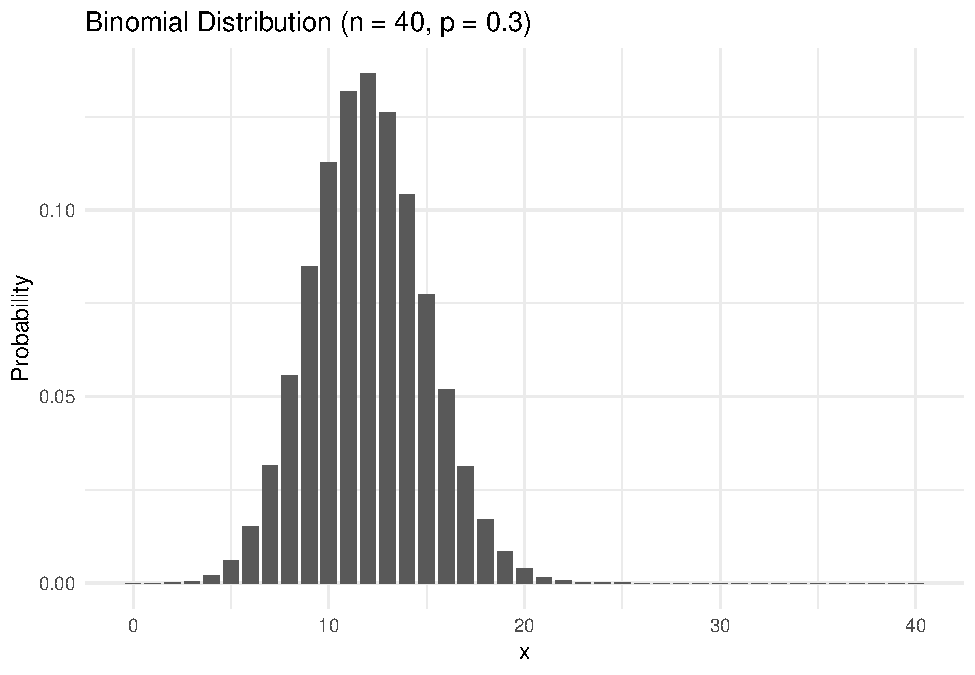
\includegraphics{Probability-Distributions_files/figure-latex/unnamed-chunk-11-1.pdf}

\hypertarget{cumulative-distribution}{%
\subsubsection{Cumulative Distribution}\label{cumulative-distribution}}

These functions are used to calculate probabilities. For example,
suppose a biochemical measure in healthy individuals is normally
distributed with a mean of 132 and a standard deviation of 13. For a
patient with a value of 160:

\begin{Shaded}
\begin{Highlighting}[]
\DecValTok{1} \SpecialCharTok{{-}} \FunctionTok{pnorm}\NormalTok{(}\DecValTok{160}\NormalTok{, }\AttributeTok{mean =} \DecValTok{132}\NormalTok{, }\AttributeTok{sd =} \DecValTok{13}\NormalTok{)}
\end{Highlighting}
\end{Shaded}

\begin{verbatim}
## [1] 0.01562612
\end{verbatim}

This indicates that approximately 1.5\% of the general population
exceeds this value. We can visualize the cumulative distribution
function of a normal distribution:

\begin{Shaded}
\begin{Highlighting}[]
\NormalTok{x }\OtherTok{\textless{}{-}} \FunctionTok{seq}\NormalTok{(}\SpecialCharTok{{-}}\DecValTok{4}\NormalTok{, }\DecValTok{4}\NormalTok{, }\FloatTok{0.1}\NormalTok{)}
\NormalTok{df\_cdf }\OtherTok{\textless{}{-}} \FunctionTok{data.frame}\NormalTok{(}\AttributeTok{x =}\NormalTok{ x, }\AttributeTok{cdf =} \FunctionTok{pnorm}\NormalTok{(x))}

\FunctionTok{ggplot}\NormalTok{(df\_cdf, }\FunctionTok{aes}\NormalTok{(}\AttributeTok{x =}\NormalTok{ x, }\AttributeTok{y =}\NormalTok{ cdf)) }\SpecialCharTok{+}
  \FunctionTok{geom\_line}\NormalTok{() }\SpecialCharTok{+}
  \FunctionTok{labs}\NormalTok{(}\AttributeTok{title =} \StringTok{"Cumulative Distribution Function of the Standard Normal Distribution"}\NormalTok{,}
       \AttributeTok{x =} \StringTok{"x"}\NormalTok{, }\AttributeTok{y =} \StringTok{"Cumulative Probability"}\NormalTok{) }\SpecialCharTok{+}
  \FunctionTok{theme\_minimal}\NormalTok{()}
\end{Highlighting}
\end{Shaded}

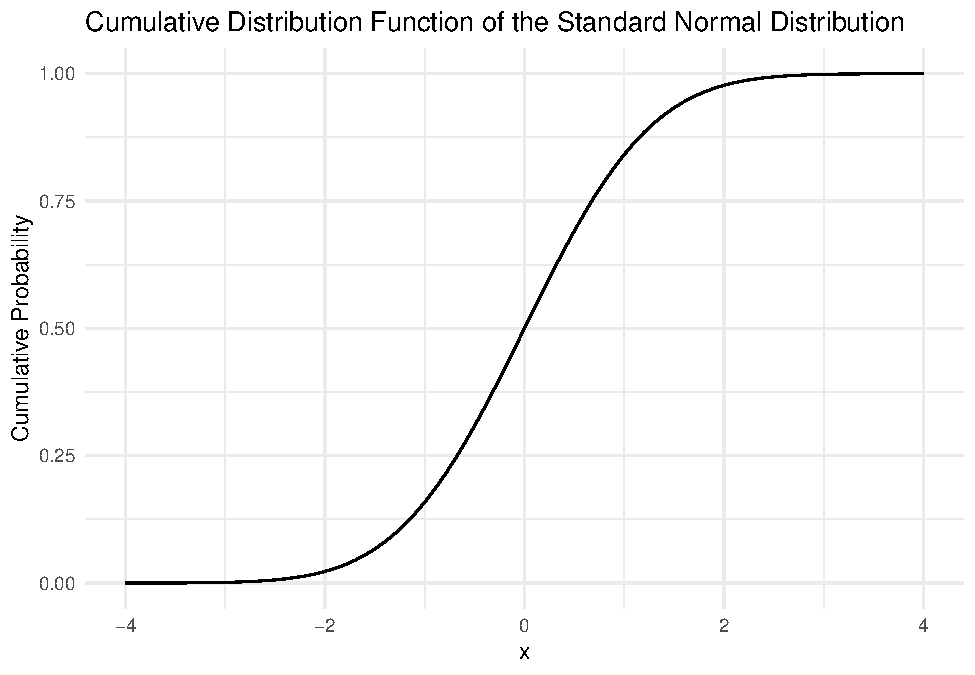
\includegraphics{Probability-Distributions_files/figure-latex/unnamed-chunk-13-1.pdf}

\hypertarget{quantiles}{%
\subsubsection{Quantiles}\label{quantiles}}

Quantile functions are the inverse of cumulative distribution functions.
For instance, to find \(z\) such that \(\Phi(z) = 0.9\):

\begin{Shaded}
\begin{Highlighting}[]
\FunctionTok{qnorm}\NormalTok{(}\FloatTok{0.9}\NormalTok{)}
\end{Highlighting}
\end{Shaded}

\begin{verbatim}
## [1] 1.281552
\end{verbatim}

\hypertarget{random-numbers}{%
\subsubsection{Random Numbers}\label{random-numbers}}

We can generate random numbers as realizations of random variables:

\begin{Shaded}
\begin{Highlighting}[]
\FunctionTok{rnorm}\NormalTok{(}\DecValTok{10}\NormalTok{, }\AttributeTok{mean =} \DecValTok{3}\NormalTok{, }\AttributeTok{sd =} \DecValTok{2}\NormalTok{)}
\end{Highlighting}
\end{Shaded}

\begin{verbatim}
##  [1] 2.048430 3.479713 3.509233 2.177056 3.245878 3.049808 4.332770 2.742566
##  [9] 1.539767 2.364050
\end{verbatim}

\begin{Shaded}
\begin{Highlighting}[]
\FunctionTok{rbinom}\NormalTok{(}\DecValTok{15}\NormalTok{, }\AttributeTok{size =} \DecValTok{50}\NormalTok{, }\AttributeTok{prob =} \FloatTok{0.2}\NormalTok{)}
\end{Highlighting}
\end{Shaded}

\begin{verbatim}
##  [1] 13 10  9  6 15  6  8  8 10 12  8 12 14  8 10
\end{verbatim}

Random data is useful for studying mathematical approximations via
simulation study.

\hypertarget{examples}{%
\subsection{Examples}\label{examples}}

\hypertarget{bernoulli-probability-model}{%
\subsubsection{Bernoulli probability
model}\label{bernoulli-probability-model}}

\textbf{Learning Experiment (Jog et al. 1999)}: To help establish neural
correlates of procedural learning, neurons in the striatum of rats are
recorded over several days as they executed a procedure learning task.
In this task, the rat used auditory cues to learn which one of two arms
of a T-maze to enter in order to receive a reward. On each trial, the
rat was placed in a T-maze. A tone was played. If it was a low tone the
animal had to go left to receive a reward, whereas if it was a high tone
it had to go right to obtain its reward. Suppose that on the previous
day, the animal executed this task 40 times and, in so doing, made 22
correct choices and 18 incorrect choices. Before, the start of the 40
trials today, what is the probability that the animal will give a
correct response on a given trial?

In this problem, there are only two possible outcomes: a correct
response or an incorrect response. The outcomes are mutually exclusive.
That is, when one outcome occurs, the other cannot occur. Let \(p\) be
the probability of a correct response.

The Bernoulli probability model would be a good model for this problem.
It defines the probability of a correct or incorrect response on each
trial. Either the quantity

\begin{Shaded}
\begin{Highlighting}[]
\NormalTok{p\_hat }\OtherTok{=} \DecValTok{22}\SpecialCharTok{/}\DecValTok{40}
\end{Highlighting}
\end{Shaded}

or \(p = 0.5\) would be a reasonable estimate (guess) of \(p\) for a
trial. Use of the parameter \texttt{p\_hat} would suggest that we expect
the performance on the trials today to be like the performance on trials
yesterday. Use of \(p = 0.5\) as the guess of \(p\) for today would
indicate a belief that performance will be indistinguishable from chance
on today's trial.

\emph{Exercise}: Plot the Bernoulli probability mass function and the
cumulative distribution.

\hypertarget{binomial-probability-model}{%
\subsubsection{Binomial probability
model}\label{binomial-probability-model}}

If today we test the rat on the same task and give it 40 trials, and we
assume that the probability of a correct choice is \(p\), what are the
possible outcomes and what is the probability of each outcome?

On each trial, there can be either a correct or an incorrect response.
Across the 40 trials, there can be any combination of correct and
incorrect responses such that the sum of correct and incorrect responses
equals 40. That is, there are \(k\) correct responses and \(40 - k\)
incorrect responses for \(k = 0,\ldots, 40\). If we assume that the
trials are independent, and that on each trial the probability of a
correct response is \(p\) and the probability of an incorrect response
is \(1-p\) then the probability of this event is
\[Pr(k \mbox{ successes}|40 \mbox{ trials}) = p^k 1-p)^{40-k}\].

\emph{Exercise}: Plot the Bernoulli probability mass function and the
cumulative distribution.

\hypertarget{poisson-probability-model}{%
\subsubsection{Poisson probability
model}\label{poisson-probability-model}}

\textbf{The Quantal Release Hypothesis} for the release of acetylcholine
at the frog motor neuromuscular junction states that in response to
stimulation, acetylcholine is released from the motor nerve terminal in
discrete ``packets'' or quanta. Normal endplate potentials (EPPs) are
the result of several hundred quanta. Miniature EPP's are the result of
spontaneous release of single quanta. An important corollary of the
quantal release hypothesis is that there is most likely a large
population of quanta in the nerve terminal, each one of which has a
small probability of being released by a nerve impulse. We now know that
these quanta are packaged in vesicles. For a fixed small time interval
(fraction of a millisecond) can we compute the probability that a given
number of quanta or vesicles will be released?

To study this problem we can formulate a binomial probability model in
which \(N\) is the number of quanta or release sites and \(p\) is the
probability of release in a given small time interval. Let us assume
that the release sites behave independently. This then leads to the
binomial probability model and hence the probability of observing
exactly \(k\) quanta released in the specified small time interval. As a
practical matter, as \(N\) becomes large, we can approximate this
calculation by assuming that the probability of release decreases so
that \(N \times p \to \lambda\). Hence, for \(N\) sufficiently large, we
have \(Np \approx \lambda\) or \(p = \frac{\lambda}{N}\).

\emph{Exercise}: Plot the Poisson probability mass function and the
cumulative distribution.

\hypertarget{exercises}{%
\section{Exercises}\label{exercises}}

\hypertarget{exercise-1}{%
\paragraph{Exercise 1}\label{exercise-1}}

Calculate the probability of each of the following events:

\begin{enumerate}
\def\labelenumi{\arabic{enumi}.}
\item
  \((X > 3)\), where \(X \sim N(0,1)\):

\begin{verbatim}
## [1] 0.001349898
\end{verbatim}
\item
  \((X > 42)\), where \(X \sim N(35,36)\):

\begin{verbatim}
## [1] 0.1216725
\end{verbatim}
\item
  \((X = 10)\), where \(X \sim Bin(10,0.8)\):

\begin{verbatim}
## [1] 0.1073742
\end{verbatim}
\item
  \((X < 0.9)\), where \(X \sim N(0,1)\):

\begin{verbatim}
## [1] 0.8159399
\end{verbatim}
\item
  \((X > 6.5)\), where \(X \sim \chi^2_2\):

\begin{verbatim}
## [1] 0.03877421
\end{verbatim}
\end{enumerate}

\hypertarget{exercise-2}{%
\paragraph{Exercise 2}\label{exercise-2}}

It is known that 5\% of the normal distribution lies outside the
interval \((-2s, 2s)\), centered at the mean. What are the corresponding
intervals for 1\%, 0.5\%, and 0.1\%? What is the position of the
quantiles expressed in terms of the standard deviation \(s\)?

\hypertarget{exercise-3}{%
\paragraph{Exercise 3}\label{exercise-3}}

Consider a disease where the probability of post-operative complications
is 20\%. A surgeon suggests a new procedure and tests it on 10 patients,
none of whom have complications. What is the probability of operating on
10 patients successfully (without complications) using the traditional
procedure?

\hypertarget{exercise-4}{%
\paragraph{Exercise 4}\label{exercise-4}}

The toss of a coin can be simulated in R using rbinom instead of sample.
How exactly can this be done?\\
Hint: Simulate 10 tosses of a fair coin using rbinom.

\hypertarget{exercise-5}{%
\paragraph{Exercise 5}\label{exercise-5}}

Suppose that we have collected the birthdays from 16 students in a
class:

\begin{longtable}[]{@{}ll@{}}
\toprule\noalign{}
\endhead
\bottomrule\noalign{}
\endlastfoot
January & 29 \\
February & 17 21 24 \\
March & 11 13 \\
April & 10 27 \\
May & 11 \\
June & 11 28 \\
July & 6 25 \\
August & 17 \\
November & 5 15 \\
\end{longtable}

Plot the probability mass function using the given sample.

\hypertarget{references}{%
\section*{References}\label{references}}
\addcontentsline{toc}{section}{References}

\hypertarget{refs}{}
\begin{CSLReferences}{1}{0}
\leavevmode\vadjust pre{\hypertarget{ref-jog1999building}{}}%
Jog, Mandar S, Yasuo Kubota, Christopher I Connolly, Viveka Hillegaart,
and Ann M Graybiel. 1999. {``Building Neural Representations of
Habits.''} \emph{Science} 286 (5445): 1745--49.

\end{CSLReferences}

\end{document}
